Text and stuff

\subsection{Scrum}

\subsubsection{Overview}

Scrum knows \textsc{3 roles}, \textsc{3 artifacts} and \textsc{5 events}.\newline

\fbox{\begin{minipage}{30em}
	Scrum \textbf{does not know} User Stories. Scrum only deals with Product Backlog Items (PBI). It is however common to use User Stories for PBIs.
\end{minipage}}

\subsubsection{3 Roles}
\begin{figure}[H] % Example image
\center{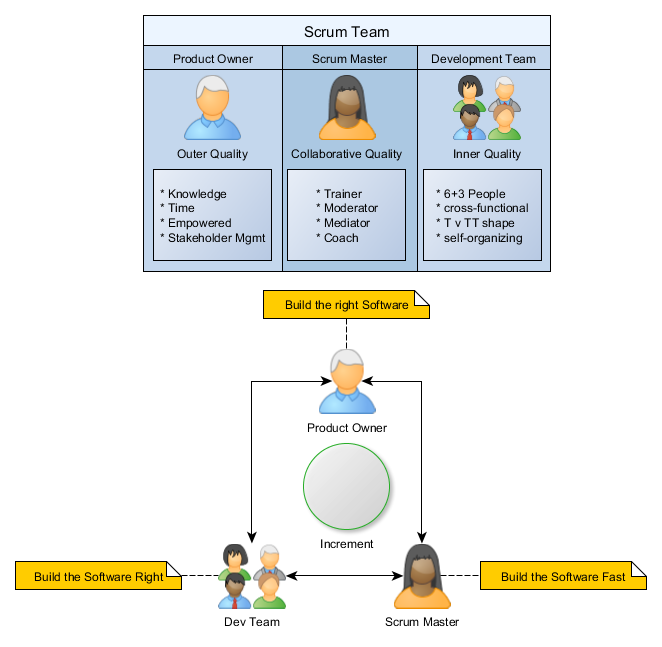
\includegraphics[width=1\linewidth]{Scrum/Roles}}
\caption{Scrum Roles}
\label{fig:scrum:roles}
\end{figure}

\paragraph{Development Team}
\begin{description}
   \item [Name] Dev Team
\end{description}
The Development Team should have a T \cite{wiki:tshaped} or $\pi$ shape. That means that the team should consist of people with a generalist (broad) skill set who are specialists in one (T-shape) specific area. Eventually that team can mature to have generlists who are specialists in two ($\pi$-shape) areas.

\subsubsection{5 Events}

\paragraph{Sprint}
\begin{description}
   \item [Name] Sprint
   \item [Herkunft] nicht Mitteleuropa
   \item [Vorkommen] Am Rand von Kornfeldern
\end{description}

\paragraph{Daily}
\begin{description}
   \item [Name] Daily Stand Up
   \item [Herkunft] nicht Mitteleuropa
   \item [Vorkommen] Am Rand von Kornfeldern
\end{description}

\paragraph{Planning}
\begin{description}
   \item [Name] Sprint Planning
   \item [Herkunft] nicht Mitteleuropa
   \item [Vorkommen] Am Rand von Kornfeldern
\end{description}

\paragraph{Review}
\begin{description}
   \item [Name] Sprint Review
   \item [Herkunft] nicht Mitteleuropa
   \item [Vorkommen] Am Rand von Kornfeldern
\end{description}

\paragraph{Retrospective}
\begin{description}
   \item [Name] Sprint Retrospective
   \item [Herkunft] nicht Mitteleuropa
   \item [Vorkommen] Am Rand von Kornfeldern
\end{description}